% !TEX root = ../notes_missingsemester.tex
% Chapter 8: Automate Everything
%%%%%%%%%%%%%%%%%%%%%%%%%%%%%%%%%%%%%%%%%%%%%%%%%%%%%%%%%%%%%%%%%%%%%%

\index{CI/CD}\index{GitHub Actions}\index{feature flag}\index{SSH}\index{systemd}
\chapter{Continuous Integration Continuous Deployment}
\printchapterversion{08_cicd_automation}
\newthought{Operation Vacation.}

% ==============================================================================================
% BLOCK 1: INTRODUCTION
% ==============================================================================================

\section{The Why}\index{automation}\index{deploy}


\newthought{Every deploy} is still a human ssh'ing into \texttt{prod}, running
\texttt{git pull}, restarting the service, and wasting a coffee break or 
feature development capacity.
The smallest tweak goes through the same heavyweight path as a real
feature, and the only gate between a push and production is the
operator's attention.

\newthought{This block closes that gap.}
A single bash script on \texttt{prod} fetches origin, runs the test
suite, and restarts the service when the tests pass.
A systemd timer fires the script every thirty seconds, so a green
commit on \texttt{main} ships without a human touching a terminal.
The end of the block introduces feature flags as the runtime switch
that lets a service change behaviour without another deploy.

\begin{figure}
\centering
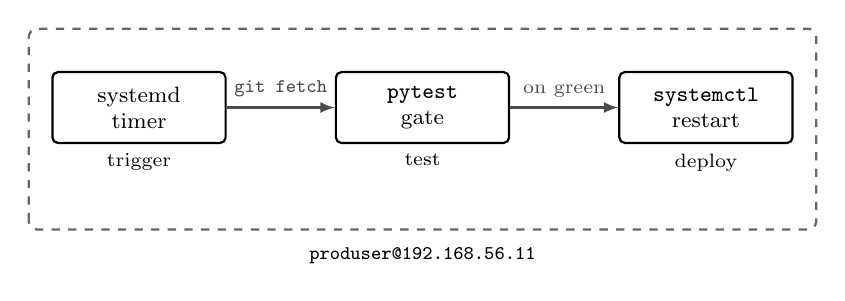
\begin{tikzpicture}[
    every node/.style={font=\footnotesize, align=center},
    box/.style={rectangle, draw=black, thick, rounded corners=2pt, minimum width=2.2cm, minimum height=0.9cm, inner sep=4pt},
    arr/.style={-latex, thick, black!70}
]
\node[box] (tim)  at (0, 0)   {systemd\\timer};
\node[box] (gate) at (3.6, 0) {\texttt{pytest}\\gate};
\node[box] (rs)   at (7.2, 0) {\texttt{systemctl}\\restart};
\draw[arr] (tim.east)  -- node[above]{\scriptsize \texttt{git fetch}}  (gate.west);
\draw[arr] (gate.east) -- node[above]{\scriptsize on green}            (rs.west);
\node[font=\scriptsize, anchor=north] at (tim.south)  {trigger};
\node[font=\scriptsize, anchor=north] at (gate.south) {test};
\node[font=\scriptsize, anchor=north] at (rs.south)   {deploy};
\draw[black!60, thick, dashed, rounded corners=3pt]
    (-1.4, -1.55) rectangle (8.6, 1.0);
\node[font=\scriptsize, anchor=north] at (3.6, -1.65) {\texttt{produser@192.168.56.11}};
\end{tikzpicture}
\caption{The classroom CI/CD cascade, all of it living on \texttt{prod}. The systemd timer is the \texttt{trigger} and fires every thirty seconds. The \texttt{test} stage fetches origin and runs \texttt{pytest} against the new commit. The \texttt{deploy} stage restarts the systemd unit, but only when the gate is green. A red test breaks the cascade before the restart.}
\label{fig:cicd_pipeline}
\end{figure}





\newthought{You wrote a fix.} Ran it locally on \texttt{dev}, it
looks right, you push to \texttt{main}, ssh to \texttt{prod}, pull,
restart, and the service is down. The fix passed your single manual check and shipped a regression
that broke the service.
No tests ran the existing endpoints, no guard sat between your push
and \texttt{prod}, and the only person who would have noticed is you.

\newthought{Every manual step} is a step a (tired) human
will skip at some point, and every skipped step is a regression waiting to ship.
Automation does not replace careful engineering: it encodes the
steps careful engineers already do, so they happen every time, in
the same order, at large-scale, without anyone remembering.


\subsection{Hands On Experience} 
\newthought{Outside the classroom.}\index{operations}
Teams call this practice DevOps.
The artefacts are different at scale, with Jenkins, GitLab CI, or
GitHub Actions runners replacing the timer, and Kubernetes
deployments replacing \texttt{systemctl restart}, but the shape is
identical: one human push, an automated gate, one observable change
to production.

\newthought{This eighth block} introduces automation around the
PixelWise pipeline.
By the end you will have
\begin{itemize}
    \item written a smoke test for \texttt{classify\_batch} that gives \texttt{pytest} something to gate on,
    \item written an auto-deploy script on \texttt{prod} that fetches origin, runs \texttt{pytest}, and restarts the service on green,
    \item registered a systemd timer that fires the script every thirty seconds,
    \item and seen how a feature flag would switch behaviour at runtime without another deploy.
\end{itemize}

\marginnote{\newthought{The pipeline is the engineering surface.}\index{pipeline}
Once a pipeline runs on every push, the test suite, the deploy
script, and the timer become part of how the application is developed. 
A good pipeline is a good engineering surface: it makes it easy to build fast and reliably.
A poor pipeline will grind you to a halt, as your code base gets more complex.}

\marginnote{\newthought{Catch up to \texttt{v0.6}.}\index{Git!tag}\index{recovery}
If \texttt{dev} or \texttt{prod} drifted from the end of Block~7,
align both machines with a hard reset to the tag:\\[0.3em]
\texttt{cd \textasciitilde/pixelwise}\\
\texttt{git fetch origin -{}-tags}\\
\texttt{git reset -{}-hard v0.6}\\
\texttt{bash setup-server.sh}\\[0.3em]
The full set of release tags lives at
\url{https://github.com/schutera/pixelwise/tags}.}


% ==============================================================================================
% BLOCK 2: CONCEPTS AND PRACTICE
% ==============================================================================================

\newpage
\section{What is CI/CD?}\index{CI/CD}\index{continuous integration}\index{continuous deployment}

\newthought{Continuous Integration, CI,} is the practice of merging
every change into a shared branch as soon as it passes an automated
gate.
The gate is a test suite that rejects broken behaviour, run on a
clean machine so the result is reproducible.
Green is safe to merge; red does not enter \texttt{main}.

\marginnote{\newthought{Deploy gate, not CI gate.}\index{CI/CD}\index{pull request}
The \texttt{pytest} step in this chapter runs on \texttt{prod} after
the push has already merged into \texttt{main}.
It gates the restart, not the merge: a red test keeps the service
on the previous green commit, but \texttt{main} already carries the
break and any developer pulling \texttt{main} pulls the break too.
A CI gate runs the same test on a pull request before the merge, so
\texttt{main} stays green by construction. We omit this step for simplicity 
and to keep the scope manageable in this lecture block.}

\newthought{Continuous Deployment, CD,} extends the chain by one
step.
The same gate that admits a commit to \texttt{main} also ships it to
production, with no human between the merge and the restart.
The unit of release shrinks from "a quarter of features" to "every
green commit on \texttt{main}", which makes each release small
enough to reason about and small enough to revert.


\newthought{Three pieces} shape every CI/CD pipeline, no matter how
elaborate the tool around them.
A trigger says when to run.
A gate says whether to proceed.
A deploy step says what to do when the gate is green.


\newthought{The industry shape.}\index{GitHub Actions}\index{Jenkins}\index{GitLab CI}
GitHub Actions, Jenkins, and GitLab CI are the cloud-hosted version
of the same idea.
A push triggers a workflow on a fresh VM the platform provisions for
the run.
The workflow installs dependencies, runs tests, and on green opens
an SSH session to production and ships the code.
The configuration lives in YAML, the runner lives somewhere else,
and usually you pay for this beyond free tiers.

\marginnote{\newthought{Bare-metal first.}\index{CI/CD}
The classroom builds the pipeline from scratch on the same machine
that hosts the service.
The trigger is a systemd timer, the gate is \texttt{pytest} on
\texttt{prod}, the deploy step is one bash script.
The substance is identical to a GitHub Actions workflow; the
difference is that every part of it is on disk in front of you,
debuggable with \texttt{journalctl}, and free.}

\newthought{The classroom shape.}\index{systemd}\index{pytest}
A single bash script on \texttt{prod} does the work.
It runs \texttt{git fetch origin}, compares the local commit hash against
\texttt{origin/main}, and exits silently if they match.
If \texttt{main} has advanced, it pulls, runs \texttt{pytest}, and
restarts the systemd unit only when the tests pass.
A systemd timer fires the script every thirty seconds, so any
commit that lands on \texttt{main} reaches \texttt{prod} before
you have switched back to the browser to check.

\newthought{What this is not.}\index{GitHub Actions}
This block does not build a GitHub Actions workflow, does not stand
up a self-hosted runner, and does not wire a webhook from the
forge into the VM.
Those are real and worthwhile patterns, and the references in this
section's margin notes describe them; the chapter teaches the
substance underneath them. In the industry this substance is usually wrapped in a hosted tool, 
which you will easily adapt to after you understand the shape here.


\newpage
\section{Exercise: The Gate or a Smoke Test}\index{exercises}\index{pytest}\index{testing}

\newthought{The gate needs something to gate on.}\index{testing!smoke}
A smoke test proves the wiring works without claiming anything about
correctness.
The name comes from electronics: turn the power on and see whether
smoke comes out.
A smoke test that fails means the code does not even run; a smoke
test that passes does not mean the code is right, only that it
runs, something we can work with.

\newthought{Where tests live.}\index{pytest}
The convention in Python is a \texttt{tests/} directory at the
repository root, with files named \texttt{test\_*.py} and functions
named \texttt{test\_*}.
\texttt{pytest} discovers them automatically; no registration, no
configuration.
The auto-deploy script in the next exercise runs
\texttt{python -m pytest tests/} from \texttt{/opt/pixelwise} and refuses to
deploy on any non-zero exit code.




\marginnote{\newthought{Go deeper later.}\index{testing}
The \texttt{pytest} documentation at
\url{https://docs.pytest.org/} is the canonical reference.
For a book-length treatment, Harry Percival's
"Test-Driven Development with Python" is free online at
\url{https://www.obeythetestinggoat.com/}.
A second testing block belongs in a follow-on course.}

\newthought{Create \texttt{tests/test\_classifier.py}} on \texttt{dev}
with a smoke test for \texttt{classify\_batch}.
The test builds a batch of two blank images, passes them through the
classifier, and asserts the response shape:

\begin{verbatim}
cd ~/pixelwise
mkdir -p tests
nano tests/test_classifier.py
\end{verbatim}

\begin{verbatim}
# tests/test_classifier.py
import numpy as np
from app.classifier import classify_batch


def test_classify_batch_returns_one_per_image():
    images = np.zeros((2, 28, 28), dtype=np.uint8)
    results = classify_batch(images)
    assert len(results) == 2


def test_classify_batch_result_shape():
    images = np.zeros((1, 28, 28), dtype=np.uint8)
    result = classify_batch(images)[0]
    assert "prediction" in result
    assert "confidence" in result
    assert isinstance(result["confidence"], float)
\end{verbatim}

\marginnote{\newthought{Two functions, one file.}\index{testing}
The first function checks the batch shape: a batch of two images
in, two results out.
The second function checks the result keys: every result is a dict
with \texttt{prediction} and \texttt{confidence}.
Together they prove the function loads, accepts the expected input,
and returns the expected shape.}

\newthought{Install \texttt{pytest} and run the test locally on
\texttt{dev}} before pushing, from the repository root so
\texttt{pytest} resolves the \texttt{app} package against the
on-disk source tree:

\marginnote{\newthought{Same gate, different trigger.}\index{CI}
The same \texttt{python -m pytest tests/} invocation that you just did locally and we will gate deployment
later is exactly what a CI runner would also execute on every pull request before merging into \texttt{main}.}

\begin{verbatim}
cd ~/pixelwise
source .venv/bin/activate
pip install pytest
python -m pytest tests/
\end{verbatim}

\marginnote{\newthought{Did it take on \texttt{dev}?}\\[0.4em]
\texttt{python -m pytest tests/} should print two passes.
If \texttt{pytest} reports an import error like
\texttt{ModuleNotFoundError: No module named 'app'},
you ran the command from the wrong directory; \texttt{cd} into
\texttt{\textasciitilde/pixelwise} and try again.
If \texttt{classify\_batch} itself fails to import, the model file
is missing on \texttt{dev}; rerun \texttt{bash setup-server.sh}.}

\newthought{Commit and push} the test.
The next exercise builds the auto-deploy script that runs the same
test on \texttt{prod} and gates the restart on it.

\marginnote{\newthought{Stage and ship.}\index{Git!commit}
\texttt{git add tests/}\\
\texttt{git commit -m "Add smoke}\\
\texttt{\ \ test for classify\_batch"}\\
\texttt{git push}}






\newpage
\section{Auto-Deploy on \texttt{prod}}\index{deploy}\index{systemd!timer}\index{bash}

\newthought{The pipeline is one bash script.}\index{automation}
The script lives in the repository and runs on \texttt{prod}.
Its body is the trigger, the gate, and the deploy step laid out in
order: fetch from origin, compare local against remote, and either
exit or pull, install, test, and restart.
A handful of operations, one shell file, version controlled like
everything else in the project.

\marginnote{\newthought{One screen, one head.}\index{bash}
A pipeline that fits on one screen fits in one head.
The deploy script is short enough to read top to bottom, the trigger
is a single timer unit, and the gate is one \texttt{pytest} call.
Everything else is an optimisation.}

\newthought{A commit hash comparison is the trigger.}\index{Git!commit hash}
The script asks Git for the local commit hash on \texttt{main} and
the remote commit hash after a fresh fetch.
Equal hashes mean nothing changed since the last run and the script
exits cheaply.
Different hashes mean a new commit landed upstream and the rest of
the script runs.
The commit hash is the cheapest test for "is there work to do".

\newthought{The gate is \texttt{pytest}.}\index{pytest}
After the pull, the script runs the test suite against the new commit.
A non-zero exit code aborts the script before the restart.
The previous service keeps running on the old commit, the operator
sees the failure in the system log, and the next run will retry
whatever the developer pushes to fix it.

\marginnote{\newthought{Idempotence and the timer.}\index{idempotence}
The script is safe to run every thirty seconds forever.
On every run where origin has not moved, it does the cheap fetch
and exits.
On every run where the tests fail, it leaves the running service
untouched.
The deploy is the side effect, not the schedule; a timer that
fires once per second would do the same work and reach the same
state, only louder.}

\marginnote{\newthought{Pushing to \texttt{main} is shipping.}\index{Git!branch}\index{pull request}\index{code review}
With auto-deploy live, every commit that lands on \texttt{main}
restarts \texttt{prod} within seconds.
A solo classroom workflow pushes straight to \texttt{main} because
the operator is also the reviewer; a team workflow does not.
The team shape is four steps:
\begin{itemize}
    \item \texttt{branch} off \texttt{main} for the change, so \texttt{main} stays untouched while you work.
    \item \texttt{commit} on the branch as often as needed; nothing reaches \texttt{prod} yet.
    \item Open a \texttt{PR} so the diff, the CI run, and a reviewer meet before the merge.
    \item \texttt{merge} into \texttt{main} only on green CI and an approving review, at which point the pipeline ships it.
\end{itemize}
With auto-deploy on, the merge is the deploy; the \texttt{PR} is
the last place to catch a regression cheap.}

\newthought{The trigger is a systemd timer.}\index{systemd!timer}
A service unit runs the script as a regular user; a timer unit
activates the service every thirty seconds.
The system survives reboots because the timer is wired into the
boot target.
Cron would do the same job with one line of a crontab; pick cron
when systemd is not available, pick a systemd timer when it is.
The substance is the same scheduler running the same script.


\newthought{Two things this design intentionally lacks.}
The timer pulls, so there is no push notification from GitHub; a
new commit waits for the next tick.
The script is local, so there is no central dashboard of recent
runs; the system journal is the dashboard.
Both gaps trade visibility for simplicity, and the trade is the
point: at this stage of the course, the goal is the substance
underneath the dashboard, not the dashboard - you usually get that as free lunch anyways, 
but it will taste better now that you know how it was prepared. 


\newpage
\section{Exercise: Build and Activate the Pipeline}\index{exercises}\index{deploy}\index{systemd!timer}

\newthought{Step~1. The trigger.}\index{systemd!timer}\index{systemd!unit}
On \texttt{dev}, author the systemd service unit and the timer unit.
Both files live in the repository and ship to \texttt{prod} on the
next pull; systemd on \texttt{prod} will read them once the
provisioner in Step~3 copies them into \texttt{/etc/systemd/system/}.
The service unit runs the script once, as \texttt{produser}, from
the working directory \texttt{/opt/pixelwise}; the timer activates
that service fifteen seconds after boot and then every thirty seconds:

\begin{verbatim}
cd ~/pixelwise
mkdir -p deploy/systemd
nano deploy/systemd/pixelwise-deploy.service
\end{verbatim}

\begin{verbatim}
[Unit]
Description=PixelWise auto-deploy
After=network-online.target

[Service]
Type=oneshot
User=produser
WorkingDirectory=/opt/pixelwise
ExecStart=/opt/pixelwise/deploy/auto-deploy.sh
\end{verbatim}

\marginnote{\newthought{\texttt{Type=oneshot}.}\index{systemd!Type}
A service unit usually models a long-running daemon; the manager
keeps the process alive and restarts it on exit.
A oneshot unit models a job that runs to completion: systemd waits
for the script to exit, records the exit code, and goes back to
sleep.
That is exactly what an auto-deploy script is.}

\begin{verbatim}
nano deploy/systemd/pixelwise-deploy.timer
\end{verbatim}

\begin{verbatim}
[Unit]
Description=Run PixelWise auto-deploy

[Timer]
OnBootSec=15s
OnUnitActiveSec=30s
Unit=pixelwise-deploy.service

[Install]
WantedBy=timers.target
\end{verbatim}

\marginnote{\newthought{\texttt{OnBootSec} vs \texttt{OnUnitActiveSec}.}\index{systemd!timer}
\texttt{OnBootSec=15s} fires the first run fifteen seconds after
boot; \texttt{OnUnitActiveSec=30s} fires each subsequent run
thirty seconds after the previous one finished.
The pair gives you a quick first check after every reboot and a
tight cadence in between, so a push to \texttt{main} reaches
\texttt{prod} before you have switched windows.
systemd accepts plain second values here, and a tick that does
nothing but \texttt{git fetch} costs the VM nothing; production
deployments tend to be slower because the gate, not the timer,
sets the floor.}






\newpage
\newthought{Step~2. The deploy step.}\index{bash}\index{automation}
Still on \texttt{dev}, author \texttt{deploy/auto-deploy.sh}.
The file ships through Git to \texttt{prod}, where the timer from
Step~1 will execute it; that is why the script's first line is
\texttt{cd /opt/pixelwise}, the path it will sit at on \texttt{prod},
not the \texttt{\textasciitilde/pixelwise} you are editing it in.
The script is the whole pipeline: fetch origin, compare local commit hash
against \texttt{origin/main}, conditionally pull, install pinned
dependencies, gate on \texttt{pytest}, restart the service on green:

\begin{verbatim}
mkdir -p deploy
nano deploy/auto-deploy.sh
\end{verbatim}

\marginnote{\newthought{\texttt{set -euo pipefail}.}\index{bash!set}
\texttt{-e} exits on any non-zero command, \texttt{-u} errors on
unset variables, \texttt{-o pipefail} fails the whole pipeline if
any stage fails.
A silent failure inside a scheduled deploy is the worst failure
mode a pipeline can have.}

\marginnote{\newthought{Why \texttt{sudo systemctl restart}?}\index{sudo}\index{systemd}
\texttt{produser} owns the code but not the service unit; restarting
a system-level unit needs root.
\texttt{setup-server.sh} drops a one-line sudoers rule into
\texttt{/etc/sudoers.d/pixelwise} that grants \texttt{produser} a
passwordless \texttt{sudo} entry for exactly this one command and
nothing else:\\[0.3em]
\texttt{produser ALL=(root) NOPASSWD: \textbackslash}\\
\texttt{\ \ /usr/bin/systemctl restart}\\
\texttt{\ \ pixelwise}\\[0.3em]
The script can do its one privileged step without holding broad
privilege.
If the rule is missing, the journal will show a password prompt
and \texttt{exit 1} on the next deploy; re-running
\texttt{setup-server.sh} reinstalls it.}


\begin{verbatim}
#!/bin/bash
# deploy/auto-deploy.sh
# Authored on dev, executed on prod by the timer.
# Pull origin/main, gate on pytest, restart
# the service on green.
set -euo pipefail

cd /opt/pixelwise

git fetch origin

LOCAL=$(git rev-parse HEAD)
REMOTE=$(git rev-parse origin/main)
if [ "$LOCAL" = "$REMOTE" ]; then
    exit 0
fi

echo "New commit on main: $REMOTE"
git pull origin main

source .venv/bin/activate
pip install -r requirements.txt > /dev/null

if ! python -m pytest tests/; then
    echo "Tests failed, refusing to deploy."
    exit 1
fi

sudo systemctl restart pixelwise
echo "Deployed: $REMOTE"
\end{verbatim}





Mark the script executable.
The executable bit travels with the file in Git, so \texttt{prod}
gets it on pull without a second \texttt{chmod}:

\begin{verbatim}
chmod +x deploy/auto-deploy.sh
\end{verbatim}











\newpage
\newthought{Step~3. Activate the pipeline.}\index{setup-server.sh}\index{prod}
Still on \texttt{dev}, teach \texttt{setup-server.sh} to install both
unit files and enable the timer.
Append a prod-only stanza so a fresh \texttt{prod} VM picks up the
service unit, the timer unit, and the enabled state without any
manual steps:

\begin{verbatim}
nano setup-server.sh
\end{verbatim}

\begin{verbatim}
# Install the auto-deploy systemd timer on prod
if [ -f "$SCRIPT_DIR/deploy/systemd/pixelwise-deploy.timer" ] \
   && command -v systemctl >/dev/null 2>&1 \
   && id produser >/dev/null 2>&1; then
    sudo cp "$SCRIPT_DIR/deploy/systemd/pixelwise-deploy.service" \
        /etc/systemd/system/pixelwise-deploy.service
    sudo cp "$SCRIPT_DIR/deploy/systemd/pixelwise-deploy.timer" \
        /etc/systemd/system/pixelwise-deploy.timer
    sudo systemctl daemon-reload
    sudo systemctl enable --now pixelwise-deploy.timer
fi
\end{verbatim}


\marginnote{\newthought{Stage and ship.}\index{Git!commit}
\texttt{git add deploy/ \textbackslash}\\
\texttt{\ \ setup-server.sh}\\
\texttt{git commit -m "Add auto-}\\
\texttt{\ \ deploy script and timer"}\\
\texttt{git push}}

\marginnote{\newthought{Did the timer install?}\\[0.4em]
On \texttt{prod}:\\
\texttt{systemctl list-timers \textbar{} grep pixelwise}\\[0.3em]
Should print one line with the next firing time, the previous run,
and the timer unit name.
If the line is missing, \texttt{systemctl status
pixelwise-deploy.timer} usually shows the reason: a typo in the
unit file, the service unit not found, or the timer not enabled.}

Stage the script, both unit files, and the updated
\texttt{setup-server.sh}, then push to \texttt{origin}.
Switch to \texttt{prod} for the last manual deploy the chapter needs.
SSH in, pull the new commit, and re-run the provisioner so the timer
and the service unit land in \texttt{/etc/systemd/system/} and the
timer starts ticking.
After this run the timer takes over and no later step in the chapter
touches \texttt{prod} by hand:

\begin{verbatim}
ssh produser@192.168.56.11
cd /opt/pixelwise
git pull
bash setup-server.sh
\end{verbatim}




\marginnote{\newthought{Read the journal like a log.}\index{journalctl}
\texttt{-u} narrows the journal to one unit.
\texttt{-f} follows it like \texttt{tail -f}, printing every new
line as the timer fires.
A pipeline you cannot read is a pipeline you cannot trust;
\texttt{journalctl} is the dashboard the timer comes with for
free.} 

Watch the pipeline live.
On \texttt{prod}, in a second shell, tail the journal for the
deploy unit.
Every run prints either a single \texttt{exit 0} line on a no-op
fetch, the new commit hash on a real deploy, or the \texttt{pytest} output
on a red run:

\begin{verbatim}
journalctl -u pixelwise-deploy -f
\end{verbatim}


\marginnote{\newthought{Did the commit land on \texttt{main}?}\\[0.4em]
After the next tick, the journal on \texttt{prod} should carry your
new hash:\\[0.3em]
\texttt{journalctl -u pixelwise-deploy}\\
\texttt{\ \ -n 5}\\[0.3em]
A \texttt{Deployed: <hash>} line that matches the hash you just
pushed means the pipeline did its job; no such line, or an older
hash, is where the chain broke. Of course you can also just check the change in the readme.}

Push a trivial commit from \texttt{dev} to see the end-to-end loop.
A whitespace change to the \texttt{README} is enough to advance the
commit hash on \texttt{main}.
The next tick of the timer picks it up, runs the tests, restarts
the service, and prints the new commit hash into the journal:

\begin{verbatim}
cd ~/pixelwise
echo "" >> README.md
git commit -am "Trivial commit to trigger auto-deploy"
git push
\end{verbatim}



\newpage
\section{Optional Exercise: Notify Discord on Deploy}\index{exercises}\index{webhook}\index{Discord}

\newthought{A webhook is an HTTP POST to a known URL.}\index{webhook}
The pipeline runs in silence; the only signal of a deploy is a
fresh commit hash in \texttt{journalctl}.
A Discord webhook makes it audible: one \texttt{curl} call appends
to a chat channel every time the script restarts the service or
refuses to.
Create one in the target channel under Integrations, Webhooks,
"New Webhook", then "Copy Webhook URL".

\marginnote{\newthought{The URL is the secret.}\index{webhook}
A Discord webhook URL ends in a long opaque token; anyone with the
URL can post to the channel.
Treat it like a password: keep it off GitHub and out of screenshots.
The variable does not land in \texttt{.env.example}; each operator
pastes their own URL into \texttt{.env} on the machine that needs
it.}

\newthought{Add the URL to \texttt{.env} on \texttt{prod}}\index{secrets}
alongside the other runtime secrets, then edit
\texttt{auto-deploy.sh} on \texttt{prod} to source \texttt{.env}
near the top and to \texttt{curl} the webhook in the
\texttt{pytest} failure branch and after the
\texttt{systemctl restart}:

\begin{verbatim}
# /opt/pixelwise/.env
DISCORD_WEBHOOK_URL="https://discord.com/api/..."

# after `cd /opt/pixelwise`
if [ -f .env ]; then
    set -a; source .env; set +a
fi

# inside the pytest failure branch
curl -sf -H "Content-Type: application/json" \
    -d "{\"content\":\"Deploy red: $REMOTE\"}" \
    "$DISCORD_WEBHOOK_URL" > /dev/null || true

# after `sudo systemctl restart pixelwise`
curl -sf -H "Content-Type: application/json" \
    -d "{\"content\":\"Deployed: $REMOTE\"}" \
    "$DISCORD_WEBHOOK_URL" > /dev/null || true
\end{verbatim}

\marginnote{\newthought{Why \texttt{|| true}?}\index{bash}
\texttt{set -e} aborts the script on any non-zero exit.
A flaky Discord call should not roll back a successful deploy or
hide a failed test; \texttt{|| true} swallows the notification's
exit so the rest of the script keeps going.
Notifications are useful, not load-bearing.}

Run the script once by hand to see the next message land in the
channel:

\begin{verbatim}
sudo -u produser bash \
    /opt/pixelwise/deploy/auto-deploy.sh
\end{verbatim}

\marginnote{\newthought{Not part of \texttt{v0.7}.}\index{automation}
The canonical \texttt{auto-deploy.sh} at \texttt{v0.7} does not
include the notification.
Push it to your own \texttt{main} if you want to keep it; just
know it is your local addition and the reference tag stays clean.}


\newpage
\section{Optional: Feature Flags}\index{feature flag}

\newthought{A feature flag is a runtime switch.}
The code path exists in the binary, but a check at the start of the
path decides whether to take it.
The check reads a boolean from \texttt{.env}, an environment
variable, or a row in a config table.
Flipping the flag changes behaviour without changing code, without
a deploy, and without a build.

\marginnote{\newthought{The shape of the flag.}\index{feature flag}
A simple flag is a boolean.
A multi-arm flag is a string from a known set, like \texttt{v1} vs
\texttt{v2}.
A percentage flag rolls a feature out to a fraction of traffic.
A targeted flag fires for one user, one cohort, one region.
The boolean is the floor; the others compose from it.\\[0.3em]
\texttt{if NEW\_UI: render\_v2()}\\
\texttt{if MODEL == "v2": ...}\\
\texttt{if random() < 0.1: ...}\\
\texttt{if user in COHORT: ...}}

\newthought{A deploy ships code; a flag ships behaviour.}
Decoupling the two is the single most useful primitive in modern
service operation: a broken feature turns off in seconds without a
rollback, a risky migration runs dark for a day before going live,
and a code path can land on \texttt{main}, pass CI, sit in
production unused, and switch on only when the dashboards are
ready to watch what it does.
A commented-out path cannot do any of that: it is invisible to the
test suite, the type checker, and any reviewer searching for
usages, where a flag-gated path is real code that compiles, runs
in CI, and lights up the moment the flag flips.

\marginnote{\newthought{Dark launch in detail.}\index{feature flag!dark launch}
The code ships to production, runs against real traffic, and
stays invisible to users because the button, page, or endpoint
that would expose it is gated off.
A new search backend runs on every query, returns its answers
into a sink, and logs latency and error rates next to the live
backend it shadows.
A new pricing engine recomputes every cart in the background
and writes its number to a log column the customer never sees.
The point is to learn from production load before any user can
notice the change: the day the surface goes live the path has
already been exercised at full scale, and the team argues from
a week of graphs rather than a guess.}

\newthought{Use cases in the wild}\index{feature flag} cover more
shapes of release than the on/off picture suggests:
\begin{itemize}
\item Progressive rollout flips a path on for a fraction of
traffic first.
\item Dark launch deploys code before the user-visible surface
is ready.
\item A kill switch keeps a wrong path gated until the fix ships.
\item An A/B experiment runs two arms in parallel and keeps the
winner.
\item A targeted flag fires only for one team's accounts so the
new path runs in real traffic before a wider audience sees it.
\end{itemize}



\marginnote{\newthought{Outside the classroom.}\index{feature flag}
Production teams use hosted flag systems like LaunchDarkly,
Unleash, or Statsig that store flags out of band and push changes
to running services in seconds.
A small project uses \texttt{.env} because it is the lightest
implementation of the same pattern; the mechanism is identical.}

\newthought{How a flag is read} matters more than what it contains.
A flag read once at import time survives until the next restart;
a flag read on every request turns on the moment the operator
edits \texttt{.env} and the next request comes in.
Small services read on every request; large services cache the
read with a short refresh to keep the hot path fast.




% ==============================================================================================
% BLOCK 3: CONSOLIDATION
% ==============================================================================================

\newpage
\section{Tag \texttt{v0.7}}\index{Git!tag}

\newthought{The pipeline is the artefact.}
The end of every block is a tagged, runnable state.
Stage every file the block added or changed, commit, push, tag, and
push the tag.
Future catch-ups reset to this tag and arrive at the same place you
are now:

\marginnote{\newthought{What lands in \texttt{v0.7}.}\index{Git!tag}
\texttt{tests/test\_classifier.py} with the smoke test;
\texttt{deploy/auto-deploy.sh} as the pipeline;
\texttt{deploy/systemd/pixelwise-deploy.service} and
\texttt{deploy/systemd/pixelwise-deploy.timer} as the trigger;
an extended \texttt{setup-server.sh} that installs both units.
The optional Discord notification and the feature flag theory do
not change the repository's tagged state.}

\begin{verbatim}
cd ~/pixelwise
git add tests/ \
    deploy/auto-deploy.sh \
    deploy/systemd/pixelwise-deploy.service \
    deploy/systemd/pixelwise-deploy.timer \
    setup-server.sh
git commit -m "End of Block 8: auto-deploy pipeline"
git tag -a v0.7 \
    -m "End of Block 8: auto-deploy script and timer"
git push --follow-tags
\end{verbatim}

\marginnote{\newthought{Watch the pipeline land its own tag.}\index{CI/CD}
The push that creates \texttt{v0.7} is a push to \texttt{main}, so
the next tick of the timer picks it up.
The script pulls the tagged commit on \texttt{prod}, runs the
tests, restarts the service, and writes the new commit hash into the
journal.
The first time a chapter ships its own deploy is a moment worth
pausing for.}

\newthought{The pipeline now runs without you.}
Every commit on \texttt{main} is tested.
Every green test ships.
The service is automated.

\newthought{Catching up to \texttt{v0.7}.}\index{Git!tag}\index{recovery}
If a future block finds either machine drifted from this state,
align both with a hard reset to the tag and a re-run of the
provisioner on \texttt{prod}.
On \texttt{dev} the tag carries the test, the script, and the unit
files into the working tree:

\begin{verbatim}
cd ~/pixelwise
git fetch origin --tags
git reset --hard v0.7
\end{verbatim}

\marginnote{\newthought{Why \texttt{setup-server.sh} again.}\index{systemd}\index{recovery}
A bare \texttt{git reset} restores the unit files inside the
repository on \texttt{prod}, but systemd reads from
\texttt{/etc/systemd/system/}.
The Block~8 additions to the provisioner copy the timer and the
service into that directory, run \texttt{systemctl daemon-reload},
and enable the timer.
Re-running the provisioner is what closes the gap between repo
state and systemd state.}

On \texttt{prod} the same reset is followed by the provisioner so
the timer and the deploy service land in \texttt{/etc/systemd/}
and the next tick of the timer picks the tag up:

\begin{verbatim}
ssh produser@192.168.56.11
cd /opt/pixelwise
git fetch origin --tags
git reset --hard v0.7
bash setup-server.sh
\end{verbatim}

The full set of release tags lives at
\url{https://github.com/schutera/pixelwise/tags}.


% ==============================================================================================

\newpage
\section{Self-Reflection and Recap}\index{reflection}\index{recap}

\newthought{Self-Reflection} questions to guide your thoughts:
\begin{itemize}
    \item A test catches a regression on a feature branch; a user catches it in \texttt{prod}. Where in the pipeline is the cheapest place to catch the next one?
    \item What kinds of regression does the smoke test against \texttt{classify\_batch} catch, and what kinds does it miss?
    \item The timer fires every thirty seconds. What property of \texttt{auto-deploy.sh} makes it safe to fire on the same commit hash again, and what breaks if that property goes away?
    \item Where does the classroom auto-deploy script differ from a GitHub Actions workflow that does the same job, and where is the substance identical?
    \item A feature flag stays \texttt{false} for three months and the code path never runs. What makes the flag-gated version safer to leave in the binary than the same code commented out?
\end{itemize}

\newthought{Recap} of key concepts:
\begin{itemize}
    \item Continuous Integration runs tests on every change against a known state; Continuous Deployment ships every green commit to \texttt{main} without a human in the loop.
    \item The classroom pipeline is three primitives: a systemd timer as the trigger, \texttt{python -m pytest tests/} as the gate, and one bash script as the deploy step.
    \item The smoke test in \texttt{tests/test\_classifier.py} doubles as the gate: a non-zero exit from \texttt{pytest} stops the deploy before \texttt{systemctl restart}.
    \item \texttt{systemctl list-timers} shows the schedule and \texttt{journalctl -u pixelwise-deploy} reads its history; swap the timer for a GitHub Actions cron and the script body barely changes.
    \item Feature flags gate code that lives in the binary, so flipping behaviour is a config edit and a restart instead of a deploy.
\end{itemize}

\marginnote{\newthought{You made it Zauberlehrling.}\index{security}
Und nun sollen seine Geister
Auch nach meinem Willen leben.
Seine Wort´ und Werke
Merkt ich und den Brauch,
Und mit Geistesstärke
Tu ich Wunder auch.}

\newthought{Milestone.}
You now own a service that ships itself.
A commit to \texttt{main} flows through tests, lands on \texttt{prod}
without a human in the loop, and tag \texttt{v0.7} marks the
pipeline itself as the artefact.
